\justifying
\begin{center}
    \section{
        \textit{Circuito I: Topologias de realimentacion positiva-negativa.}
    }
\end{center}

Se debe sintetizar un filtro pasa banda de cuarto orden con la plantilla de requerimientos de la figura.

Con ayuda de PYTHON y mediante una aproximacion de Chebychev, se obtuvieron las funciones de transferencia a sintetizar:

\begin{figure}[H]
    \centering
    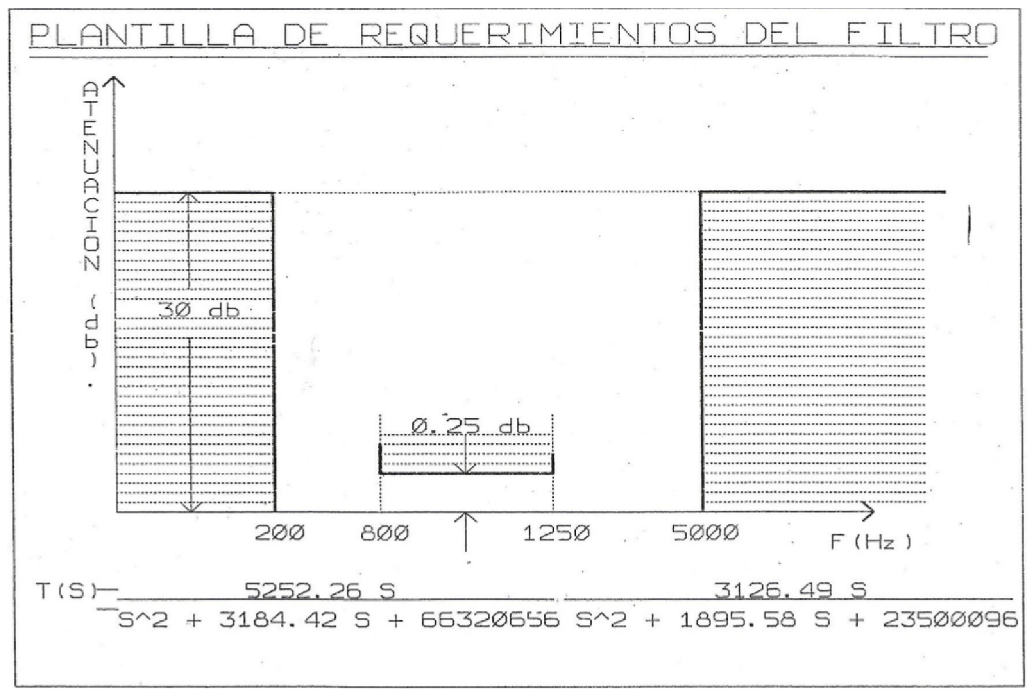
\includegraphics[scale=.3]{Secciones/Circ1/img/plantilla.png}
    \caption{Requerimientos y resultados de la aproximacion.}
    \label{prop}
\end{figure}

Para realizar un analisis completo de topologias, aprender de la experiencia y utilizar todas las herramientas, se decidio dividir la respuesta del filtro en 2 funciones de transferencia en cascada e implementar una con topologia canonica de realimentacion positiva (Sallen-Key), la otra con topologia canonica de realimentacion negativa y agregar un aplificador inversor final como ajuste de ganancia. 

En ambos casos se utilizo el metodo de igualacion de coeficientes con las sugerencias del libro ''Principles of Active Network Synthesis and Design'', de Gobind Daryanani (en adelante ''El Daryanani''). \\

\textit{NOTA AL PIE: Es claro que incluir un amplificador inversor adicional es contraproducente ya que se agrega una etapa y no se cumple la idea de ''la menor cantidad de amplificadores''. 
Si bien esto se evita sintetizando ambas etapas con topologias del mismo tipo, se considero como objetivo principal analizar y aprender sobre ambas topologias utilizando la mayor cantidad de herramientas.}

\textit{... se tomo ''el camino largo'' en pos de hacer el analisis mas completo.}